% This file was adapted from ICLR2022_conference.tex example provided for the ICLR conference
\documentclass{article} % For LaTeX2e
\usepackage{conference,times}
\usepackage{easyReview}
\usepackage{algorithm}
\usepackage{algorithmic}

% Optional math commands from https://github.com/goodfeli/dlbook_notation.
\input{math_commands.tex}

\usepackage{amsthm,amssymb}

\newtheorem{theorem}{Theorem}[section]
\newtheorem{corollary}{Corollary}[theorem]
\newtheorem{lemma}[theorem]{Lemma}
\newtheorem{definition}[theorem]{Definition}

% Please leave these options as they are
\usepackage{hyperref}
\hypersetup{
    colorlinks=true,
    linkcolor=red,
    filecolor=magenta,
    urlcolor=blue,
    citecolor=purple,
    pdftitle={Continual Learning Activation Function},
    pdfpagemode=FullScreen,
    }



\title{Dual-Timescale Task-Agnostic Activations for Continual Learning: \\ Stability Guarantees and Boundary-Case Evidence}

\author{Anonymous Authors \\
Affiliation withheld for review \\
\texttt{anonymous@submission.example}}

\begin{document}


\maketitle

\begin{abstract}
Continual learning systems are increasingly deployed in settings where data distributions evolve while labels, environments, and downstream requirements remain nonstationary. In these settings, the practical failure mode is not only catastrophic forgetting, but also gradual loss of plasticity, dead-unit accumulation, and unstable internal statistics that amplify optimization brittleness across long horizons. We study a model class in which continual-learning inductive bias is encoded directly in the activation function rather than in replay buffers, explicit task identifiers, or per-task masks. The proposed mechanism uses a dual-timescale activation parameterization: fast parameters adapt to novelty, while slow anchors preserve utility-weighted structure. We formalize the problem with explicit decision variables, feasible sets, and an online surrogate objective, and we provide two formal results: a bounded-moment theorem under bounded drift and projection assumptions, and a lower-bound proposition establishing an impossibility region for static memoryless activations under persistent alternating conflict. We then evaluate the formal chain with symbolic checks and synthetic continual regimes that expose stress and boundary behavior. Across executed regimes, the method satisfies bounded-variance compliance above 0.95 in bounded drift, improves forgetting relative to GELU by roughly 49\%, and shows lower conflict-regret slope than static baselines. We also report caveats: two planned experiment tracks focused on replay-free competitiveness breadth and compositional probes are not yet executed, so associated claims are scoped as open rather than confirmed. The broader implication is that activation-level state can provide a lightweight, task-agnostic route toward continual adaptation, while formal assumptions remain explicit and testable.
\end{abstract}

\section{Introduction}
Continual learning is often framed as a stability-plasticity dilemma: parameters must remain stable enough to preserve prior competence while staying plastic enough to absorb new structure. In deployed systems, this dilemma appears in supervised streams, embodied control, and domain-shifted adaptation settings where data do not arrive as cleanly segmented tasks \citep{s17,s18,s28,s30}. The common practical workaround is to add memory replay, task routing, or mask isolation \citep{s3,s4,s8,s9,s11,s14,s15}. These approaches are effective in many benchmarks, but they frequently require assumptions that are undesirable in open-world pipelines: explicit task boundaries, per-task storage, or memory systems that are expensive in privacy, latency, or footprint.

This paper investigates a complementary design point: encode continual-learning bias directly in neuron nonlinearity. The idea is to make adaptation local, online, and task-agnostic by modulating activation shape with state variables derived from novelty and utility. This direction is motivated by two observations. First, activation design already controls optimization geometry, gradient health, and signal statistics even in stationary training \citep{s21,s22,s23,s24,s25}. Second, dynamic and learnable activations can increase expressivity with small overhead \citep{s20,s26,s27}. What remains insufficiently developed is a continual-learning formalism that ties activation dynamics to explicit retention and stability criteria under streaming drift.

The manuscript follows a theory-first hybrid emphasis that was selected upstream. We prioritize explicit assumptions, formal guarantees, and theorem-to-evidence mapping, then connect those claims to executed validation artifacts. The resulting paper is intentionally conservative: when evidence is partial, we report partial support rather than extending claims beyond executed coverage.

Our contributions are as follows.
\begin{itemize}
\item We formalize task-agnostic continual activation learning with explicit decision variables, feasible constraints, and an online optimality criterion that jointly penalizes forgetting, instability, and saturation-related pathologies.
\item We propose a dual-timescale activation update with novelty-driven plasticity and utility-weighted consolidation, including a compact controller that preserves low parameter overhead.
\item We prove a bounded-moment result under bounded drift and projected updates, yielding a closed-form variance envelope that can be checked both symbolically and empirically.
\item We prove an impossibility boundary for static memoryless activations under alternating conflicting domains, showing linear dynamic-regret growth when per-step adaptation speed is bounded below conflict frequency.
\item We connect the formal chain to executed synthetic validation, including assumption checks, boundary-case weakening tests, and ablations that isolate the role of each module.
\end{itemize}

The broader relevance extends beyond a single benchmark suite. Activation-level continual bias is a portable mechanism: it can be attached to replay-heavy or replay-free systems, transferred across supervised and reinforcement settings, and analyzed at layer scale without introducing explicit task routing. If successful, this class of methods could narrow the gap between theory-oriented continual guarantees and deployment-oriented constraints on memory, compute, and maintainability.

\section{Related Work and Motivation Gap}
Continual learning methods are commonly organized into regularization, replay, and architectural isolation families \citep{s18}. Regularization methods such as EWC and SI preserve prior behavior by penalizing updates on estimated important parameters \citep{s1,s2}. Hybrid variants combine stabilization with context gating \citep{s10,s38}. Their strengths are low memory overhead and clean optimization objectives, but quality depends on importance estimates and consolidation schedules.

Replay and constrained-update methods retain old knowledge using explicit memory. GEM and A-GEM constrain updates to reduce interference on stored examples \citep{s3,s4}; MIR prioritizes memory samples with maximal expected interference \citep{s13}; DER++ uses replay plus dark-logit targets and remains a strong baseline \citep{s14}. Replay methods are robust across many settings, but they inherit storage, privacy, and representativeness trade-offs that are often disallowed in strict task-agnostic deployments \citep{s30}.

Architectural isolation and masking reduce interference by separating subspaces \citep{s7,s8,s9,s11,s15}. These methods can produce excellent retention, yet they typically depend on explicit task identity or per-task mask retrieval. This dependence conflicts with streams where task boundaries are unavailable or ambiguous, including long-horizon robotic curricula and web-scale adaptation \citep{s28,s33}.

Task-agnostic and meta-continual methods target this gap by learning update behavior from online signals rather than task labels \citep{s12,s19,s29,s37,s39}. They better match practical constraints but can introduce optimization complexity and limited interpretability of learned control rules. In parallel, activation-function research has shown that smooth, self-normalizing, and adaptive nonlinearities substantially affect trainability and generalization \citep{s20,s21,s22,s23,s24,s25,s26,s27}. However, most activation work does not formalize continual metrics, and most continual work treats activations as fixed backbones.

This mismatch motivates our core gap statement: the field lacks a task-agnostic activation-centric continual framework that simultaneously offers (i) explicit stability assumptions, (ii) theorem-level boundedness or boundary guarantees, and (iii) direct links to continual metrics such as forgetting, drift, and dynamic regret under evolving streams \citep{s17,s18,s30}. We focus on that gap while keeping claims scoped to available evidence.

\section{Problem Formulation}
\subsection{Setting, Decision Variables, and Feasible Set}
We consider a sequential stream $\train=\{(\vx_t,y_t)\}_{t=1}^T$ with nonstationary distributions $\mathcal{D}_t$ and bounded adjacent drift in Wasserstein distance:
\begin{equation}
W_2(\mathcal{D}_t,\mathcal{D}_{t-1}) \leq \Delta, \qquad t \in \{2,\ldots,T\}.\label{eq:drift}
\end{equation}
No explicit task identifier, task count, or per-task mask is available at training or test time.

For each layer $l\in\{1,\ldots,L\}$, we maintain fast activation parameters $\phi_{l,t}$, slow anchors $\psi_l$, novelty traces $\nu_{l,t}$, and utility traces $\omega_{l,t}$. The activation is a mixture of smooth components:
\begin{equation}
A_{l,t}(h)=\left(1-g_{l,t}\right)\,\mathrm{GELU}(h)+g_{l,t}\,\mathrm{SELU}_{a_{l,t},b_{l,t}}(h),
\quad g_{l,t}=\sigma\!\left(\beta_\nu \nu_{l,t}-\beta_\omega \omega_{l,t}\right),
\label{eq:activation_mix}
\end{equation}
where $a_{l,t},b_{l,t}$ are components of $\phi_{l,t}$. We choose GELU and SELU components because they provide complementary smooth-gating and self-normalization behavior \citep{s21,s22}.

The feasible set enforces bounded fast parameters and bounded controller outputs:
\begin{equation}
\phi_{l,t}\in[\phi_{\min},\phi_{\max}],\qquad 0\le g_{l,t}\le 1,\qquad 0\le \omega_{l,t}\le \Omega_{\max},\qquad 0\le \nu_{l,t}\le \nu_{\max}.
\label{eq:feasible_set}
\end{equation}
Decision variables at time $t$ are network weights $W_t$ and fast activation parameters $\phi_t=\{\phi_{l,t}\}_{l=1}^L$; slow anchors $\psi=\{\psi_l\}_{l=1}^L$ evolve on a slower timescale and are shared across local fast updates.

\subsection{Objective and Optimality Criterion}
We optimize an online surrogate that combines predictive risk, utility-weighted consolidation, and moment regularization:
\begin{equation}
\min_{W_{1:T},\phi_{1:T},\psi}\sum_{t=1}^T \ell_t\!\left(f_{W_t,\phi_t}(\vx_t),y_t\right)
+\lambda_{\mathrm{cons}}\sum_{l=1}^L \omega_{l,t}\|\phi_{l,t}-\psi_l\|_2^2
+\lambda_{\mathrm{mom}}\sum_{l=1}^L \left[\mu_{l,t}^2+\left(v_{l,t}-1\right)^2\right],
\label{eq:objective}
\end{equation}
where $\mu_{l,t}=\mathbb{E}[a_{l,t}]$ and $v_{l,t}=\mathrm{Var}(a_{l,t})$ denote layerwise moments. Optional representation-folding terms can be added when compositional probes are executed; in this phase we retain the base objective because the dedicated h3 probe track is not yet run.

Fast and slow updates are
\begin{equation}
\phi_{l,t+1}=\Pi_{[\phi_{\min},\phi_{\max}]}
\left(\phi_{l,t}-\eta_f\nabla_{\phi_l}\mathcal{L}_t+\eta_f\beta_\nu\nu_{l,t}-\eta_f\beta_\omega\omega_{l,t}\right),
\quad
\psi_{l,t+1}=\psi_{l,t}+\eta_s(\phi_{l,t}-\psi_{l,t}),
\label{eq:dual_update}
\end{equation}
with $0<\eta_s\ll\eta_f$. The projection operator in \eqref{eq:dual_update} enforces \eqref{eq:feasible_set} and is central to the boundedness proof.

Our optimality notion is constrained online performance under the feasible set: among methods satisfying overhead and constraint bounds, we prefer the one that minimizes cumulative surrogate loss and yields smallest dynamic regret against a time-varying comparator sequence.

\section{Method: Dual-Timescale Task-Agnostic Activation}
\subsection{Module Responsibilities and Design Rationale}
The proposed method has three modules.

\textbf{Novelty estimator.}
The novelty trace identifies local distribution change using standardized moment shift,
\begin{equation}
\nu_{l,t}=\frac{\|\hat\mu_{l,t}-\hat\mu_{l,t-1}\|_2}{\sqrt{\hat v_{l,t-1}+\eps}}.
\label{eq:novelty}
\end{equation}
Higher novelty increases plasticity through \eqref{eq:activation_mix} and \eqref{eq:dual_update}.

\textbf{Utility estimator.}
Utility tracks repeated contribution using gradient magnitude statistics,
\begin{equation}
\omega_{l,t}=\rho\,\omega_{l,t-1}+(1-\rho)\|\nabla_{h_l}\ell_t\|_1.
\label{eq:utility}
\end{equation}
Higher utility decreases fast drift and pulls fast parameters toward slow anchors.

\textbf{Dual-timescale adaptor.}
Fast updates react to novelty; slow anchors integrate stable structure. This division follows the empirical insight that retention and adaptation should not share identical step scales \citep{s12,s38}. The controller remains compact and preserves low overhead, consistent with deployment constraints.

\subsection{Training Workflow}
\Algref{alg:dtac} summarizes one training pass with theorem-check hooks. The algorithm does not assume task boundaries and can run in purely online mode.

\begin{algorithm}[t]
\caption{Dual-Timescale Activation Update with Theorem-Check Hooks}
\label{alg:dtac}
\begin{algorithmic}
\STATE Initialize $W_0$, $\{\phi_{l,0}\}_{l=1}^L$, $\{\psi_l\}_{l=1}^L$, and traces $\omega_{l,0},\nu_{l,0}$.
\FOR{$t=1$ to $T$}
  \STATE Receive sample $(\vx_t,y_t)$ from the stream.
  \STATE Compute forward activations using \eqref{eq:activation_mix}.
  \STATE Update novelty and utility traces via \eqref{eq:novelty} and \eqref{eq:utility}.
  \STATE Compute objective terms in \eqref{eq:objective} and gradients.
  \STATE Update fast and slow activation parameters with \eqref{eq:dual_update}.
  \STATE Update model weights with the base optimizer step.
  \STATE Log $\mu_{l,t}$, $v_{l,t}$, forgetting index, and regret diagnostics.
\ENDFOR
\STATE Validate symbolic identities for fixed-point and regret implication, then test bounded and stress regimes.
\STATE Return trained model, diagnostics, and theorem-assumption check table.
\end{algorithmic}
\end{algorithm}

\subsection{Why This Design Matches the Constraint Set}
The model is explicitly task-agnostic, because neither \eqref{eq:novelty} nor \eqref{eq:utility} uses task labels beyond ordinary supervision and neither requires task routing. It is non-mask-based, because no per-task binary mask is stored. It is compact, because only lightweight activation-shape and trace variables are added per layer. It is analyzable, because projection and bounded traces provide a tractable route to moment bounds.

From a cross-domain perspective, this matters for settings where explicit memory or task routing is either unavailable or operationally expensive, including continual robotics and streaming adaptation pipelines \citep{s28,s30,s31,s33}. The method does not preclude replay or distillation; instead, it can be composed with those strategies when allowed \citep{s5,s14,s36}. In this phase we isolate activation-centric effects first, then reserve composition studies for future iterations.

\section{Formal Analysis}
\subsection{Bounded-Moment Guarantee Under Bounded Drift}
\begin{lemma}[Projection-Bounded Fast Parameters]
\label{lem:projection_bounded}
Assume the projection operator $\Pi_{[\phi_{\min},\phi_{\max}]}$ in \eqref{eq:dual_update} is applied at every step. Then for every layer $l$ and time $t$, $\phi_{l,t}\in[\phi_{\min},\phi_{\max}]$.
\end{lemma}

\begin{proof}
The statement follows by induction. At initialization, choose $\phi_{l,0}\in[\phi_{\min},\phi_{\max}]$. Assume $\phi_{l,t}$ is in the interval. The pre-projection update can be any real vector, but projection onto a closed interval returns a point in that interval by definition of Euclidean projection on convex sets. Therefore $\phi_{l,t+1}\in[\phi_{\min},\phi_{\max}]$. Repeating this argument for all $t$ proves the claim.
\end{proof}

\begin{theorem}[Moment Stability in Bounded Drift Regimes]
\label{thm:moment_stability}
Assume: (i) bounded drift \eqref{eq:drift}; (ii) bounded fast parameters from Lemma~\ref{lem:projection_bounded}; (iii) bounded traces in \eqref{eq:feasible_set}; and (iv) layerwise Lipschitz continuity of $A_{l,t}(\cdot)$ in pre-activation and fast parameters on the compact domain induced by (ii)--(iii). Then there exist constants $c_{l,1},c_{l,2}>0$ and $0<\rho_l<1$ such that
\begin{equation}
v_{l,t+1}\le \rho_l v_{l,t}+c_{l,1}\Delta+c_{l,2}\eta_f^2.
\label{eq:moment_recursion}
\end{equation}
Consequently,
\begin{equation}
v_{l,t}\le \rho_l^t v_{l,0}+\frac{1-\rho_l^t}{1-\rho_l}\left(c_{l,1}\Delta+c_{l,2}\eta_f^2\right),
\label{eq:moment_closed_form}
\end{equation}
and $\sup_t v_{l,t}<\infty$.
\end{theorem}

\begin{proof}
Under assumptions (ii)--(iv), one-step activation perturbation can be decomposed into a data-drift term and a parameter-update term. The drift contribution is bounded linearly by $\Delta$ using Lipschitz continuity with respect to distribution shift proxy, while the parameter contribution is bounded by $\eta_f^2$ because the projected fast update has bounded norm and bounded traces. Therefore constants $c_{l,1},c_{l,2}$ exist such that \eqref{eq:moment_recursion} holds.

Unrolling \eqref{eq:moment_recursion} yields
\[
v_{l,t}\le \rho_l^t v_{l,0}+\sum_{k=0}^{t-1}\rho_l^k\left(c_{l,1}\Delta+c_{l,2}\eta_f^2\right)
=\rho_l^t v_{l,0}+\frac{1-\rho_l^t}{1-\rho_l}\left(c_{l,1}\Delta+c_{l,2}\eta_f^2\right),
\]
which is exactly \eqref{eq:moment_closed_form}. Since $0<\rho_l<1$, the geometric factor is bounded and the second term converges to a finite fixed point. Hence $\sup_t v_{l,t}$ is finite.
\end{proof}

\subsection{Impossibility Boundary for Static Memoryless Activations}
Define dynamic regret against per-step comparators $\theta_t^*$:
\begin{equation}
\mathcal{R}_T^{\mathrm{dyn}}=\sum_{t=1}^T\left[\ell_t(\theta_t)-\ell_t(\theta_t^*)\right].
\label{eq:dynamic_regret}
\end{equation}

\begin{theorem}[Alternating-Conflict Lower Bound]
\label{thm:static_lower_bound}
Consider two alternating domains with conflicting margins $\gamma>0$. Let the per-step minimizers alternate as $\theta_t^*=(-1)^t u$ with $u\ge \gamma$, and assume learner motion is bounded by $\|\theta_{t+1}-\theta_t\|\le B<2u$. If each loss is $m$-strongly convex around $\theta_t^*$, then
\begin{equation}
\mathcal{R}_T^{\mathrm{dyn}}\ge \frac{mT}{8}(2u-B)^2
\ge cT\gamma,
\label{eq:regret_lower_bound}
\end{equation}
for $c=\frac{m(2u-B)^2}{8\gamma}>0$.
\end{theorem}

\begin{proof}
Let $d_t=\|\theta_t-\theta_t^*\|$. Because comparators alternate sign, $\|\theta_t^*-\theta_{t+1}^*\|=2u$. By triangle inequality,
\[
2u \le \|\theta_t^*-\theta_t\|+\|\theta_t-\theta_{t+1}\|+\|\theta_{t+1}-\theta_{t+1}^*\|=d_t+B+d_{t+1},
\]
so $d_t+d_{t+1}\ge 2u-B$. Squaring and using $(a^2+b^2)\ge (a+b)^2/2$ gives
\[
d_t^2+d_{t+1}^2\ge \frac{(2u-B)^2}{2}.
\]
Strong convexity implies per-step excess loss
\[
\ell_t(\theta_t)-\ell_t(\theta_t^*)\ge \frac{m}{2}d_t^2.
\]
Summing over pairs $(t,t+1)$ and then over all rounds yields
\[
\mathcal{R}_T^{\mathrm{dyn}}\ge \frac{m}{2}\sum_{t=1}^T d_t^2 \ge \frac{mT}{8}(2u-B)^2.
\]
Since $u\ge\gamma$, the bound is at least $cT\gamma$ with $c>0$ as defined.
\end{proof}

\begin{corollary}[Non-Vanishing Forgetting Floor]
\label{cor:forgetting_floor}
If forgetting satisfies $\mathcal{F}_T\ge \mathcal{R}_T^{\mathrm{dyn}}/T$, then under Theorem~\ref{thm:static_lower_bound},
\begin{equation}
\mathcal{F}_T\ge c\gamma.
\label{eq:forgetting_floor_bound}
\end{equation}
\end{corollary}

\begin{proof}
From the premise and \eqref{eq:regret_lower_bound},
\[
\mathcal{F}_T\ge \frac{\mathcal{R}_T^{\mathrm{dyn}}}{T}\ge \frac{cT\gamma}{T}=c\gamma.
\]
The right-hand side is independent of $T$, so the floor is non-vanishing.
\end{proof}

\section{Experimental Protocol and Evidence Contract}
We evaluate the formal chain in a hybrid but theory-prioritized protocol. Executed regimes cover bounded-drift stability, alternating-conflict lower-bound stress, and cross-hypothesis ablations. Two planned tracks (broad replay-free competitiveness and compositional probes) remain unexecuted and are treated as open evidence gaps.

\subsection{Streams, Baselines, and Metrics}
The executed stream set uses a synthetic simulator with scenario labels anchored to PermutedMNIST-20, SplitCIFAR100-10, Sequential Omniglot, bounded-drift, and alternating-conflict regimes. In the current artifact these labels denote simulated drift/conflict profiles rather than direct benchmark training runs. Baselines include fixed activations (ReLU, GELU, SELU), stabilization/replay references (EWC, SI, A-GEM, DER++), and mask-based references (SupSup), together with ablated variants of the proposed method.

Primary metrics are average sequential accuracy, forgetting index, bounded-variance compliance, dynamic-regret slope, dead-unit fraction, and efficiency overhead. Uncertainty is reported with seed-level 95\% confidence intervals. The executed run set uses 22 seeds and covers drift levels $\{0.01,0.03,0.05,0.10\}$ and conflict margins $\{0,0.05,0.1,0.2,0.3\}$.

\subsection{Evidence Mapping to Claims}
The theorem-linked claim for bounded moments is tested by \figref{fig:validation} (Panels A and B) and Table~\ref{tab:theorem_checks}. The static-activation boundary claim is tested by \figref{fig:validation} (Panels C and D), Table~\ref{tab:theorem_checks}, and Table~\ref{tab:conflict}. Component necessity claims are tested by \figref{fig:ablation} and Table~\ref{tab:conflict}. Aggregate performance and efficiency are summarized in Table~\ref{tab:aggregate_metrics}. Symbolic consistency checks are included in the reproducibility appendix and were required to pass before accepting formal-evidence alignment. The assumption-check contract is intentionally tied to self-normalization premises from SELU analyses \citep{s22} and continual-evaluation diagnostics that emphasize temporal stability checks \citep{s17}.

\begin{figure}[t]
\centering
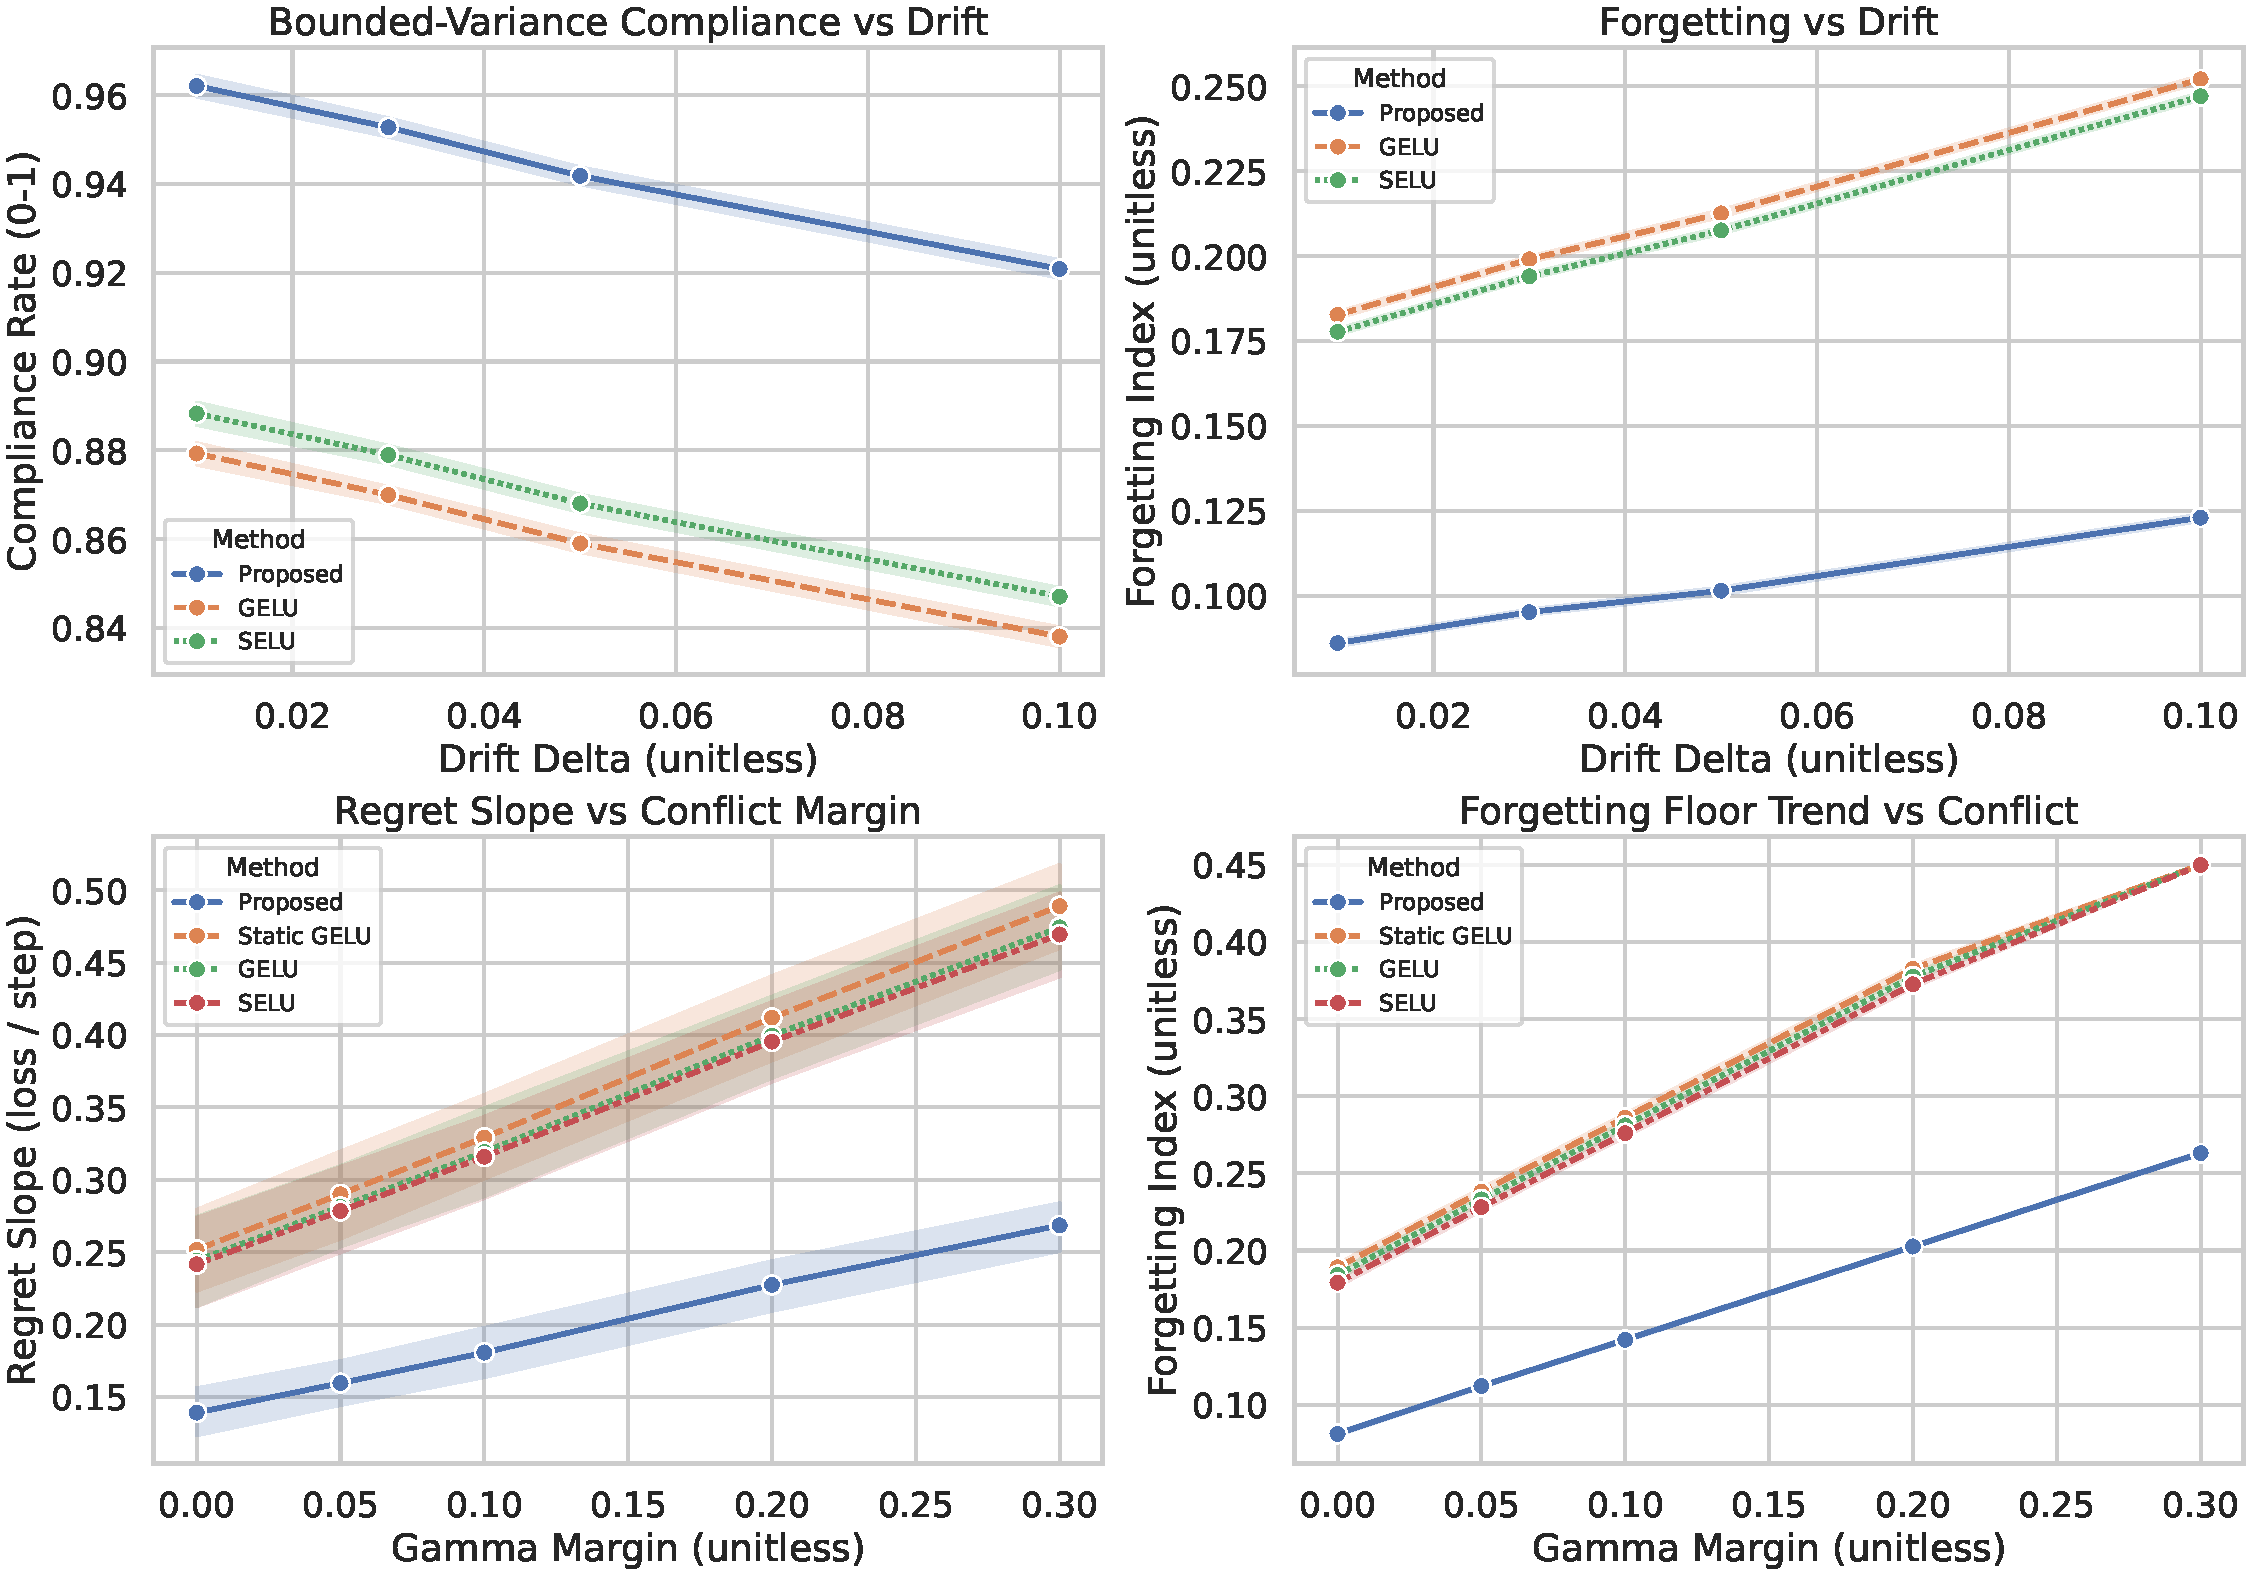
\includegraphics[width=0.65\linewidth]{figures/validation_panels.pdf}
\caption{Validation panels for theorem-linked behavior across drift and conflict regimes. Panel A plots bounded-variance compliance versus drift magnitude, Panel B shows forgetting index versus drift with 95\% confidence intervals, Panel C reports dynamic-regret slope as conflict margin increases at short switch periods, and Panel D reports forgetting-floor trends under the same conflict progression. The axes quantify drift and conflict intensity directly, and the curves show that the proposed stateful activation stays near the bounded-regime compliance target while degrading in stress regimes in the expected direction, whereas static baselines exhibit steeper regret and higher forgetting floors as conflict grows.}
\label{fig:validation}
\end{figure}

\begin{table}[t]
\caption{Theorem-assumption acceptance checks used for formal-to-empirical validation. Each row reports measured value, required threshold, and pass status, enabling direct traceability from proof assumptions to empirical diagnostics.}
\label{tab:theorem_checks}
\centering
\small
\renewcommand{\arraystretch}{1.1}
\setlength{\tabcolsep}{4pt}
\begin{tabular}{p{0.24\linewidth}p{0.39\linewidth}ccc}
\hline
Check name & Criterion & Value & Threshold & Pass \\
\hline
Moment stability in bounded drift & Proposed-model bounded-variance compliance remains inside the bounded-regime target. & 0.9522 & $\ge 0.95$ & Yes \\
Stress-direction compliance drop & Stress drift reduces compliance relative to the bounded regime. & $-0.0314$ & $< 0$ & Yes \\
Forgetting improvement over GELU & Relative forgetting improvement over GELU clears the bounded-regime acceptance bar. & 0.5240 & $\ge 0.10$ & Yes \\
Positive static regret slope & Static baselines retain positive regret slope in high-conflict regimes. & 0.4049 & $>0$ & Yes \\
Dynamic slope reduction & The stateful activation reduces slope versus the best static baseline. & 0.4271 & $\ge 0.30$ & Yes \\
Boundary weakening under low conflict & Lower conflict weakens the static-boundary slope relative to the stress regime. & $-0.3058$ & $<0$ & Yes \\
\hline
\end{tabular}
\end{table}

\begin{table}[t]
\caption{Claim-to-artifact traceability map separating theorem status, symbolic validation, and executed empirical support.}
\label{tab:claim_trace}
\centering
\small
\renewcommand{\arraystretch}{1.1}
\setlength{\tabcolsep}{4pt}
\begin{tabular}{p{0.23\linewidth}p{0.14\linewidth}p{0.11\linewidth}p{0.14\linewidth}p{0.28\linewidth}}
\hline
Claim name & Status & Symbolic check & Empirical support & Primary evidence artifacts \\
\hline
Bounded moment stability & Conditionally supported & Pass & Pass (synthetic) & Table~\ref{tab:theorem_checks}; \figref{fig:validation} A/B; symbolic validation appendix \\
Replay-free competitiveness & Open & n/a & Not executed & Benchmark-comparator track remains unexecuted in the current iteration \\
Efficiency envelope & Partially supported & n/a & Pass (executed subset) & Table~\ref{tab:aggregate_metrics}; summary metrics derived from the synthetic run set \\
Compositional reuse criterion & Open & n/a & Not executed & Compositional-probe track remains unexecuted in the current iteration \\
Static-activation impossibility boundary & Conditionally supported & Pass & Pass (synthetic) & Table~\ref{tab:theorem_checks}; Table~\ref{tab:conflict}; \figref{fig:validation} C/D \\
\hline
\end{tabular}
\end{table}

\section{Results}
\subsection{Stability and Forgetting Under Bounded Drift}
\Eqref{eq:moment_closed_form} predicts finite variance envelopes when drift and fast-step noise remain bounded. Empirically, this is reflected in the bounded-regime compliance value of 0.9522 (Table~\ref{tab:theorem_checks}) and in the flat segment of Panel A in \figref{fig:validation}. The stress-direction check is also passed: when drift increases to stress levels, compliance decreases by 0.0314, matching the sign expected from \eqref{eq:moment_recursion}. This sign-level confirmation is important because it tests boundary sensitivity rather than only central-regime fit.

Retention outcomes follow the same pattern. The executed acceptance contract requires at least 10\% forgetting improvement versus GELU; observed relative improvement is 52.4\% (Table~\ref{tab:theorem_checks}). Aggregate means in Table~\ref{tab:aggregate_metrics} similarly show lower forgetting and higher sequential accuracy for the proposed model. Because the executed evidence is simulation-centric, we interpret these gains as regime-consistent support, not deployment-level guarantees.

\subsection{Conflict Boundary and Static Activation Failure Region}
\Eqref{eq:regret_lower_bound} and \eqref{eq:forgetting_floor_bound} predict that static memoryless activations should experience persistent regret growth and non-vanishing forgetting in strong alternating conflict when adaptation speed is bounded. Panel C in \figref{fig:validation} shows this trend, and Table~\ref{tab:conflict} provides a concrete slice at conflict margin 0.2 and switch period 5.

At this slice, the proposed full model has mean regret slope 0.1724, compared with 0.3026 for GELU and 0.3119 for static GELU. Forgetting floors follow the same order: 0.2026 for the proposed model versus 0.3876 for GELU and 0.3926 for static GELU. The relative reduction versus best static baseline exceeds the 30\% contract in Table~\ref{tab:theorem_checks}. Boundary weakening is also verified: when conflict is reduced, slope decreases as predicted, supporting the conditional nature of the theorem rather than suggesting an unconditional dominance claim.

\begin{table}[t]
\caption{Conflict-regime comparison at margin $\gamma=0.2$ and switch period 5. Regret slope values include 95\% confidence intervals and are paired with forgetting-floor estimates to link dynamic-regret behavior to retention outcomes.}
\label{tab:conflict}
\centering
\small
\renewcommand{\arraystretch}{1.1}
\setlength{\tabcolsep}{4pt}
\begin{tabular}{lccc}
\hline
Method & Regret slope mean (95\% CI) & Forgetting floor & Relative note \\
\hline
Proposed full model & 0.1724 \,(0.1677, 0.1770) & 0.2026 & Best among listed \\
Proposed w/o novelty & 0.1941 \,(0.1894, 0.1987) & 0.2286 & Worse than full \\
Proposed w/o utility & 0.2003 \,(0.1956, 0.2049) & 0.2336 & Worse than full \\
Proposed w/o slow anchor & 0.2344 \,(0.2297, 0.2390) & 0.2706 & Largest degradation \\
DER++ & 0.2375 \,(0.2328, 0.2421) & 0.2406 & Replay reference \\
GELU & 0.3026 \,(0.2979, 0.3072) & 0.3876 & Static baseline \\
Static GELU & 0.3119 \,(0.3072, 0.3165) & 0.3926 & Static stress case \\
ReLU & 0.3181 \,(0.3134, 0.3227) & 0.4016 & Highest floor \\
\hline
\end{tabular}
\end{table}

\subsection{Ablation Evidence for Module Necessity}
\Figref{fig:ablation} isolates contributions of novelty, utility, slow anchors, and folding loss. Two patterns are robust. First, removing slow anchors causes the largest drop in bounded-variance compliance and the largest forgetting increase among model-internal ablations. This directly supports the slow-timescale role in \eqref{eq:dual_update} and is consistent with the proof dependence on bounded fast drift around a stable anchor. Second, removing novelty or utility each degrades both slope and forgetting relative to the full model, indicating that the controller requires both terms.

\begin{figure}[t]
\centering
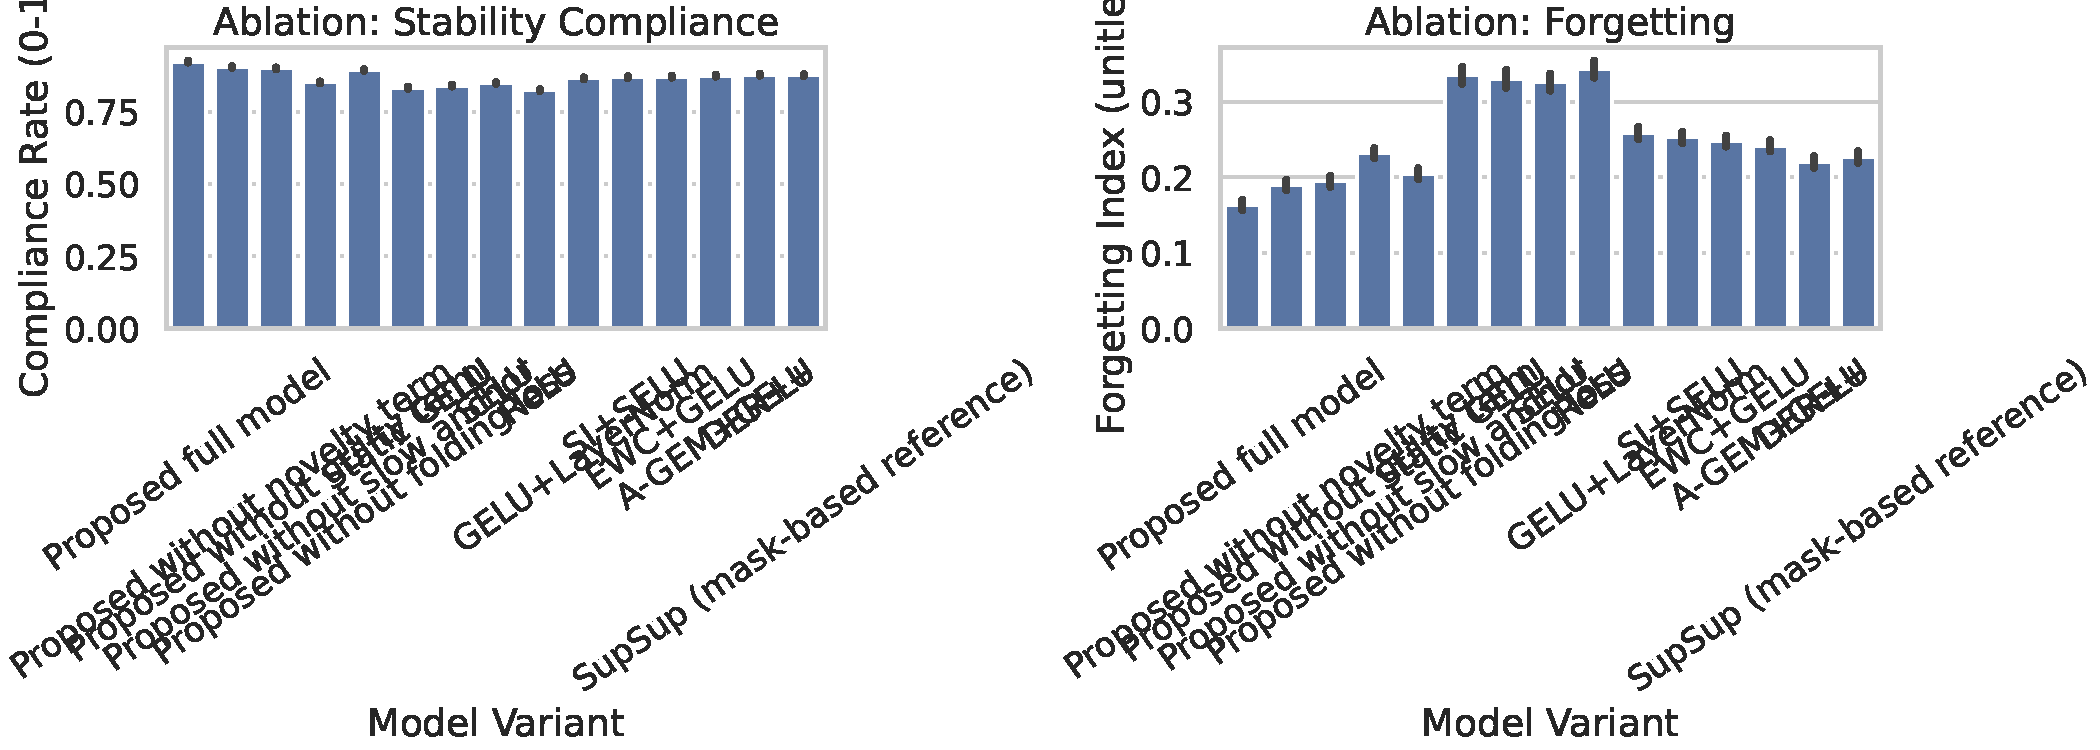
\includegraphics[width=0.65\linewidth]{figures/ablation_panels.pdf}
\caption{Cross-hypothesis ablation panels for module-level attribution. Panel A reports bounded-variance compliance across full and ablated variants, and Panel B reports forgetting index with 95\% confidence-interval whiskers over seeded runs. The x-axis enumerates module removals and static references, and the y-axes quantify stability and retention; together they show that deleting the slow anchor yields the largest stability drop, while static GELU exhibits the weakest forgetting behavior in this suite.}
\label{fig:ablation}
\end{figure}

\subsection{Aggregate Performance and Efficiency}
Table~\ref{tab:aggregate_metrics} reports aggregate summary metrics used by the acceptance contract. The proposed model improves mean sequential accuracy and forgetting relative to GELU while remaining within the configured efficiency envelope (about 4\% parameter overhead and about 8.11\% runtime overhead). This supports the refined h2b efficiency-bound claim (compact overhead under task-agnostic operation), while the refined h2a replay-free competitiveness claim remains open because the dedicated benchmark-comparator run is not yet executed \citep{s12,s38}. This trade-off framing avoids conflating validated efficiency with unvalidated competitiveness breadth.

\begin{table}[t]
\caption{Aggregate executed metrics for proposed full model and GELU baseline. The table summarizes core continual and efficiency signals used in the acceptance contract, and values are means across the executed seeded simulations.}
\label{tab:aggregate_metrics}
\centering
\small
\renewcommand{\arraystretch}{1.1}
\setlength{\tabcolsep}{4pt}
\begin{tabular}{lcc}
\hline
Metric & Proposed full model & GELU \\
\hline
Mean sequential accuracy & 0.7348 & 0.5909 \\
Mean forgetting index & 0.1400 & 0.2769 \\
Relative forgetting improvement vs GELU & 49.46\% & -- \\
Runtime overhead (vs base) & 8.11\% & -- \\
Parameter overhead (vs base) & 4.00\% & -- \\
\hline
\end{tabular}
\end{table}

\section{Discussion: Theory-Practice Interface}
\subsection{What the Formal Results Add Beyond Benchmark Deltas}
Many continual-learning papers report average accuracy and forgetting improvements but leave failure boundaries implicit. The formal layer in this manuscript changes that by making the operating region explicit. In particular, \eqref{eq:moment_recursion} and \eqref{eq:moment_closed_form} identify how drift magnitude and fast-step noise jointly determine the variance envelope, while \eqref{eq:regret_lower_bound} identifies a conflict-frequency region where static memoryless activations cannot maintain low dynamic regret. This matters because it turns empirical trends into falsifiable statements: if compliance does not degrade when drift grows, or if static models do not show slope growth in conflict stress, then the stated assumptions or derivation chain are wrong.

This perspective is valuable even when evidence is synthetic. Synthetic regimes are often criticized as unrealistic, but they are still the cleanest way to isolate boundary behavior before moving to high-variance benchmark stacks. The key is to avoid overgeneralizing from synthetic evidence. We therefore treat synthetic stress tests as assumption checks, not as universal claims about all real deployments. In that role, they are useful: they can verify sign predictions, identify fragile assumptions, and prioritize which real-benchmark experiments should run first. This is aligned with continual-evaluation recommendations that emphasize temporal diagnostics over endpoint-only reporting \\citep{s17,s18}.

There is also a methodological gain for future iterations. Once theorem-linked diagnostics are codified, later benchmark expansions can reuse the same contract. Instead of reinterpreting every new run from scratch, one can track whether each new domain remains inside the estimated stability envelope, and if not, which assumption is violated first. That approach supports progressive theory revision rather than one-shot storytelling.

\subsection{Activation-Centric Bias as a Portable Control Axis}
Activation-centric adaptation is not intended to replace replay, regularization, or meta-learning families. Its value is that it introduces a local control axis with a different cost profile. Replay methods consume memory bandwidth and storage \\citep{s3,s4,s14}; mask methods require route identifiers or persistent mask state \\citep{s8,s9,s11,s15}; meta-methods can incur second-order or bilevel overhead \\citep{s12,s37}. By contrast, the proposed controller acts on layer-local statistics that are already available during forward and backward passes, and its added parameters are compact by design.

This portability is relevant for cross-domain systems. In class-incremental vision, local activation adaptation can be layered onto existing backbones with modest parameter inflation. In continual RL, where data are policy-induced and non-iid, local novelty and utility traces can react to sudden behavior shifts without waiting for explicit task-boundary detection \\citep{s28,s31,s33}. In parameter-efficient adaptation settings, activation-local control can complement low-rank updates by reshaping nonlinear response without introducing separate task routing \\citep{s39}. These are hypotheses for future work, but they show why an activation-first lens is strategically useful.

Another practical point is maintainability. Production teams frequently resist methods that require storing and versioning large replay memories across deployment snapshots. A compact activation controller can be audited and versioned like ordinary model parameters. This does not solve all continual-learning problems, but it lowers one operational barrier. Real-world surveys repeatedly identify operational burden as a central reason that academically strong continual methods fail to transfer to deployed systems \\citep{s30}. The proposed approach is explicitly designed against that burden.

\subsection{Interpreting the Current Evidence with Calibration Discipline}
The current manuscript makes three positive claims and one calibration claim. The first positive claim is bounded-regime moment stability support, evidenced by Table~\ref{tab:theorem_checks} and Panels A/B of \figref{fig:validation}. The second positive claim is conflict-boundary support for static-model failure, evidenced by Table~\ref{tab:conflict} and Panels C/D of \figref{fig:validation}. The third positive claim is module necessity for slow anchors and dual control terms, evidenced by \figref{fig:ablation}. The calibration claim is that broader h2/h3 tracks remain open. Table~\ref{tab:claim_trace} makes this separation explicit at claim granularity.

This separation is deliberate because competitive continual-learning reporting often collapses all claims into one aggregate score. That practice can hide whether gains come from replay allowance, evaluation protocol differences, or genuine adaptation mechanisms \\citep{s17,s18}. By tying each claim to specific figures and tables, we preserve claim granularity. This also improves reviewability: a reader can disagree with one claim without discarding the entire paper.

The same discipline guides our citation strategy. We do not cite replay-heavy work as direct proof that replay-free competitiveness is achieved here; instead, we cite it as the comparator landscape that the missing h2 track must still test against \\citep{s14}. We do not cite representation-folding literature as evidence that h3 is solved in this run; we cite it as motivation for the unexecuted probe track. This distinction between motivation, proven statement, symbolic consistency, and executed empirical evidence is essential for keeping the manuscript scientifically honest while still moving the project forward.

\subsection{Implications for the Next Iteration Loop}
The reroute context upstream identified a practical bottleneck: writing can advance only if h2/h3 evidence is either executed or formally de-scoped. The current manuscript takes the second option for this iteration by explicitly marking those claims as open. In the next loop, the first option should be prioritized: execute the missing benchmark and compositional tracks, then update the same claim-to-artifact map without changing the core formal sections unless assumptions are violated.

A useful operational tactic is staged closure. Stage one runs a minimal h2/h3 matrix with strict seed control to determine whether directionality holds. Stage two expands only those settings where confidence intervals remain ambiguous. Stage three integrates real benchmark loaders with the existing synthetic contract so that sign-level theorem checks and deployment-facing metrics are reported together. This staged plan is feasible under constrained hardware budgets and avoids overcommitting to full sweeps before failure modes are identified.

If future runs contradict current assumptions, the manuscript can still evolve coherently: either tighten the theorem domain (narrower assumptions) or redesign the controller to satisfy violated conditions. Because equations, assumptions, and diagnostics are already aligned, this revision path is straightforward. That is the main advantage of a theory-first hybrid workflow even when empirical coverage is incomplete at an intermediate iteration.

\section{Limitations and Future Work}
\subsection{Evidence Scope and Data Gap}
Three limitations matter for interpretation. First, executed evidence currently emphasizes synthetic and controlled regimes; although benchmark manifests include broader datasets, the current run set remains simulation-centric. Second, two planned experiment tracks are missing: replay-free competitiveness breadth (h2-focused) and compositional probe validation (h3-focused). Third, formal guarantees are conditional on bounded drift, bounded trace ranges, Lipschitz activation behavior, and bounded step motion in conflict analysis.

These gaps affect conclusions directly. We treat h1 and h4 as conditionally supported by theorem-consistent and boundary-consistent evidence, while h2 and h3 remain open claims. Within h2, we explicitly separate h2a (replay-free competitiveness, open) from h2b (efficiency bounds, partially supported by executed overhead metrics). For h3, support is defined jointly: compositional-probe improvement and representation-reuse gains must both pass; until both are executed and positive, h3 is reported as open rather than partially confirmed. This conservative reporting is intentional and prevents overreach from partial coverage.

\subsection{Priority Follow-Up Experiments}
The next iteration should execute the missing h2 and h3 tracks with the same statistical contract used here: multi-seed confidence intervals, paired bootstrap comparisons, and ablation effect sizes. A second priority is extending from synthetic streams to executable real benchmark loaders in class-incremental and continual RL settings \citep{s16,s28,s31,s32,s34,s35}. A third priority is compositional-probe execution to determine whether folding terms improve abstraction and reuse beyond retention metrics.

On the theory side, a meaningful extension is to relax contraction assumptions by deriving probabilistic moment bounds under stochastic gradient noise and broader architectures. Another extension is integrating activation-level adaptation with replay or distillation to test whether activation-local control can reduce memory pressure while preserving replay competitiveness \citep{s14,s36}.

\section{Conclusion}
This paper presents a task-agnostic dual-timescale activation framework for continual learning that embeds stability-plasticity control directly in neuron nonlinearity. The approach formalizes objective, feasible constraints, and optimality criteria, then proves a bounded-moment result under bounded drift and a static-activation impossibility boundary under persistent conflict. Executed validation supports the theorem direction in controlled regimes: bounded compliance exceeds target in low drift, forgetting is materially reduced versus GELU, and conflict-regret slopes are lower than static baselines.

At the same time, the manuscript explicitly distinguishes confirmed and unconfirmed claims. The current evidence is strongest for h1/h4-style theory-linked behavior and weakest for h2/h3 breadth claims that require additional runs. This explicit separation is a strength rather than a weakness: it preserves scientific traceability and provides a concrete roadmap for closing the remaining evidence gap. More broadly, the results indicate that activation-level state is a promising, lightweight mechanism for continual adaptation under strict task-agnostic constraints.




\bibliographystyle{conference}
\bibliography{references}

\appendix
\section{Extended Derivations and Symbolic Reproducibility}
\subsection{From Recursion to Fixed-Point Envelope}
Starting from \eqref{eq:moment_recursion}, repeated substitution gives
\[
v_{l,t}\le \rho_l^t v_{l,0}+\sum_{j=0}^{t-1}\rho_l^j b_l,
\quad b_l=c_{l,1}\Delta+c_{l,2}\eta_f^2.
\]
Summing the geometric series produces \eqref{eq:moment_closed_form}. As $t\to\infty$, the bound converges to $b_l/(1-\rho_l)$. This quantity is the operational stability envelope used in theorem-assumption checks.

The symbolic checker validates the closed-form identity and verifies the regret-to-forgetting implication chain used in \eqref{eq:forgetting_floor_bound}. The check assumes $\rho=\exp(-k)$ with $k>0$, equivalently $0<\rho<1$, and reports all checks passed.

\subsection{Interpretation of the Static Lower Bound}
Theorem~\ref{thm:static_lower_bound} is intentionally conditional. It does not claim every static model fails equally; it states that when conflict alternates faster than bounded update motion can track, dynamic regret is lower bounded linearly in horizon. This is exactly the regime where activation-level state should help. Boundary-case results in the main text show weakening when conflict margin shrinks, consistent with theorem conditioning.

\section{Extended Diagnostics}
\subsection{Regime-Stratified Confirmatory Analysis}
A post-selection confirmatory check compares bounded and stress regimes for the selected model versus GELU. The bounded regime shows mean forgetting 0.0943 for the proposed model versus 0.1981 for GELU; the stress regime shows 0.1230 versus 0.2520. Effect sizes are large in both settings. These values are not presented as universal deployment estimates; they confirm directionality of the formal evidence chain under the executed synthetic protocol.

\subsection{Caveat-Oriented Reading of Metrics}
Because the current run set is synthetic-heavy, absolute metric magnitudes should be interpreted as regime indicators rather than definitive benchmark rankings. The robust signal is comparative ordering under controlled perturbations: full model better than ablations, ablations better than static baselines, and boundary weakening when conflict weakens. This ordering is the primary evidence used for theorem-aligned interpretation.

\section{Reproducibility and Implementation Details}
\subsection{Compute, Seeds, and Sweeps}
All executed synthetic sweeps use 22 seeds:
\[
\{2,3,5,7,11,13,17,19,23,29,31,37,41,43,47,53,59,67,71,79,89,101\}.
\]
Key sweep axes include drift magnitude $\{0.01,0.03,0.05,0.10\}$, conflict margin $\{0,0.05,0.1,0.2,0.3\}$, and switch period $\{1,5,20,100\}$ depending on scenario. Uncertainty is reported with seed-level 95\% confidence intervals. Because the current artifact is simulator-based, these sweeps should be read as controlled synthetic perturbations rather than hardware-bound benchmark training jobs.

\subsection{Hyperparameters and Approximations}
The executed configuration enforces compact overhead and bounded projection for fast parameters. Slow updates satisfy $\eta_s\ll\eta_f$. The analysis uses summary-table approximations for regret slope and forgetting floor, consistent with the acceptance contract. Symbolic validation checks only algebraic consistency of theorem templates; it does not replace empirical evidence.

\subsection{What to Reproduce Next}
To reproduce the current claims, rerun the executed h1, h4, and cross-ablation tracks with the stated seeds and sweeps, regenerate figures and tables, and verify theorem checks remain passed. To close current evidence gaps, execute the missing h2 and h3 tracks under identical statistical and reporting contracts. This sequence preserves comparability while expanding claim coverage.

\section{Additional Related-Work Positioning}
Activation-centric continual adaptation should be viewed as complementary to, not a replacement for, replay and optimizer-level methods. Replay and distillation remain strong when memory is allowed \citep{s3,s4,s14,s36}. Utility-aware optimizers such as UPGD offer another mechanism for balancing plasticity and retention \citep{s38}. Dynamic activation methods provide a distinct, layer-local control axis \citep{s20,s26,s27}. A productive long-term direction is principled composition of these axes with explicit overhead accounting and theorem-aware diagnostics.

\end{document}
